\chapter{Results}\label{ch:results}
We now describe the results of testing the ILP systems. We conducted the experiments in accordance with the methods described in chapter \ref{ch:methodology}.

To recap the research questions are as follows:
\begin{itemize}
	\item \textbf{Q1} - Does varying the quality of game traces influence the ability for learners to solve the IGGP problems? Specifically, does the quality of game play affect predictive accuracy?
	\item \textbf{Q2} - Does varying the amount of game traces influence the ability for learners to solve the IGGP problems? Specifically, does the quality of game play affect predictive accuracy?
	\item \textbf{Q3} - Can we improve the performance of a learner by mixing the quality of traces?
\end{itemize}

Experiment \textbf{E1} answers questions Q1 and Q3 and experiment \textbf{E2} answers question Q2.

\section{Results summary}



\subsection{E1: Varying the quality of game traces}
For questions Q1 and Q3 we preform experiment E1 where we train and test each system on random and intelligent traces as well as a 50/50 mixture of both. Table \ref{tab:E1-BA} shows the average balanced accuracy of each test of the systems in E1. Table \ref{tab:E1-P} shows the number of games for which the rule was perfectly learned for each test. The the differences for each system in the average balanced accuracy for the different training/testing combinations were unpronounced. To show this we use the $\chi^2$ (chi squared) test to calculate the statistical significance of our results. The biggest difference between any two balanced accuracy testing results between two distributions for a single system was for Aleph where it was trained on Sancho traces and tested on Random (balanced accuracy of 65) and tested on Sancho (balanced accuracy of 72). The $\chi^2$ test was performed on these two scores. The result was a p-value of 0.6723. This value is well above any reasonable threshold for statistical significance meaning the results can be viewed as not significant. Despite this there are still differences worth discussing between the different results.

\begin{table}[]
	\begin{tabular}{|c|c|c|c|c|c|c|}
		\hline
		\multicolumn{7}{|c|}{Balanced Accuracy}                                                                           \\ \hline
		\multirow{2}{*}{Systems} & \multicolumn{2}{c|}{Random} & \multicolumn{2}{c|}{Sancho} & \multicolumn{2}{c|}{Mixed} \\ \cline{2-7}
		& Random       & Sancho       & Random       & Sancho       & Random       & Sancho      \\ \hline
		Metagol                  & 51           & 51           & 51           & 51           & 51           & 51          \\ \hline
		Aleph                    & 66           & 65           & 65           & 72           & 67           & 66          \\ \hline
		ILASP                    & 72           & 72           & 71           & 72           & 73           & 73          \\ \hline
	\end{tabular}
	\caption{The average balanced accuracies across all games and predicates for each system in E1. Each row gives the balanced accuracies of one system. Each was trained on random, Sancho generated and mixed traces then tested against random and Sancho generated. The top of the two header rows gives the training distribution and the lower gives the test distribution}
	\label{tab:E1-BA}
\end{table}


\begin{table}[]
	\begin{tabular}{|c|c|c|c|c|c|c|}
		\hline
		\multicolumn{7}{|c|}{Perfectly Solved}                                                                            \\ \hline
		\multirow{2}{*}{Systems} & \multicolumn{2}{c|}{Random} & \multicolumn{2}{c|}{Sancho} & \multicolumn{2}{c|}{Mixed} \\ \cline{2-7}
		& Random       & Sancho       & Random       & Sancho       & Random       & Sancho      \\ \hline
		Metagol                  & 0            & 0            & 0            & 0            & 0            & 0           \\ \hline
		Aleph                    & 1            & 0            & 0            & 4            & 1            & 0           \\ \hline
		ILASP                    & 7            & 8            & 5            & 10           & 5            & 8           \\ \hline
	\end{tabular}
	\caption{The number of perfectly solved scores for each system trained and tested as described in E1}
	\label{tab:E1-P}
\end{table}

\subsubsection{Aleph}
Throughout all experiments conducted the programs learned by Aleph consisted almost entirely of a disjunction of all cases seen in testing. For example when learning the \textit{goal} predicate it relates every board state it sees with the goal value it has and adds it to the generated program. It appears that the most general clause (see section \ref{sec:aleph}) that could be found for a lot of the examples was also the most specific clause. This simplistic method resulted in programs that performed better when the training and testing data was closely matched. This can be seen in the results for Aleph when trained and tested on Sancho generated traces. For some games all Sancho generated traces were the same, in \textit{fizz buzz} Sancho always says the correct thing and in the \textit{prisoner dilemma} both Sancho players always defect. This allowed Aleph to achieve a perfect score on the \textit{next} predicate. In cases where the training data is diverse Aleph learns a program that over approximates the solution doing well on the tests with positive examples and badly on the tests with negative examples.

Generally Aleph was best at learning the \textit{goal} predicate. Unlike \textit{next} which takes a game state and player moves as input the \textit{goal} predicate often only takes the player role. The limited number of output values, 0 to 100, also meant the output space was smaller than the other predicates. The program Aleph produced would often simply associate each role to all the different goal values it had at any point in the training data. This is a subsection of the goal values it learned for \textit{checkers}:
\begin{verbatim}
goal(red,0).
goal(black,0).
goal(black,8).
goal(red,8).
\end{verbatim}
This method does not capture the original game rule at all but achieves reasonable scores in testing.

Aleph did not do particularly better when trained on the mixed training set. It achieved similar scores to the other tests apart from when it was trained and tested on optimal traces.

\subsubsection{Metagol}
A limitation with the Metagol system is that if it cannot learn a rule that covers 100\% of the positive training examples and 0\% of the testing examples it will not output any rule at all. With the time limitations placed on the experiments due to limits in computational resources Metagol rarely managed this. If some rule contains a special case such as \textit{castling} in \textit{checkers} Metagol may have learned the general \textit{next} predicate but would not give any output since this case was not covered. The search space scales exponentially with the size of the rules to be learned.\af{check}

Metagol never learned any \textit{legal} or \textit{goal} predicates. The \textit{goal} predicate is often relatively complex. It can rely on game concepts which would be obvious to humans but hard to learn for an ML system. For example the idea of three of the same symbol in a row, column or diagonal. There might not be enough training examples to guide Metagol to concepts such as these. The \textit{legal} predicate is usually even more complex than the goal, however in some cases it the possible legal moves were constant across all states. It is possible that the metarules supplied to Metagol for this experiment were not ideal for this task.

Where Metagol learned the \textit{next} predicate it often only managed the simple parts of it. The predicate is split up into different parts such as \textit{next\_state} and \textit{next\_step} to reflect the different predicates that change each move. If one of the predicates was \textit{next\_step(N)} where \textit{N} increased by 1 each turn Metagol managed to learn that however it failed to produce any program that was more than two or three lines long.

\subsubsection{ILASP}
ILASP performed by far the best out of the three systems. The differences in results between the systems trained on Sancho and random data was not large. Out of them it scored the best when trained and tested on Sancho traces presumably for the same reasons that Aleph did (the testing data was very similar to training data). The margin by which this scored better however was almost negligible. There was generally less than 2\% difference between the balanced accuracies for each predicate of each game.

ILASP scored several percentage points better across the board when trained on the mixed data. ILASP benefited the most from the combination of training data out of all the systems. It scored better on the \textit{goal} and \textit{next} predicates but not on the \textit{legal} predicate (compared to the Sancho and random trained systems). This makes sense because the legal predicate changes the least between the optimal and random traces, the same complexity of rule still generally has to be learned in each. The \textit{next} predicate for \textit{tic tac toe} was learned a lot better by ILASP on the mixed data. It is unclear exactly why this is the case but it does appearer ILASP learns better with greater diversity of examples. 


\subsection{E2: Varying the amount of game traces}
In experiment E2 each system was trained three times on mixed traces. The first time with a total of 8 traces, the second with 16 traces and the third with 24 traces. When designing this experiment it was assumed that the more traces they were given to train on the better the systems would perform. However, as can been see in the scatter graph of the results this was not the case.
\\\\\\
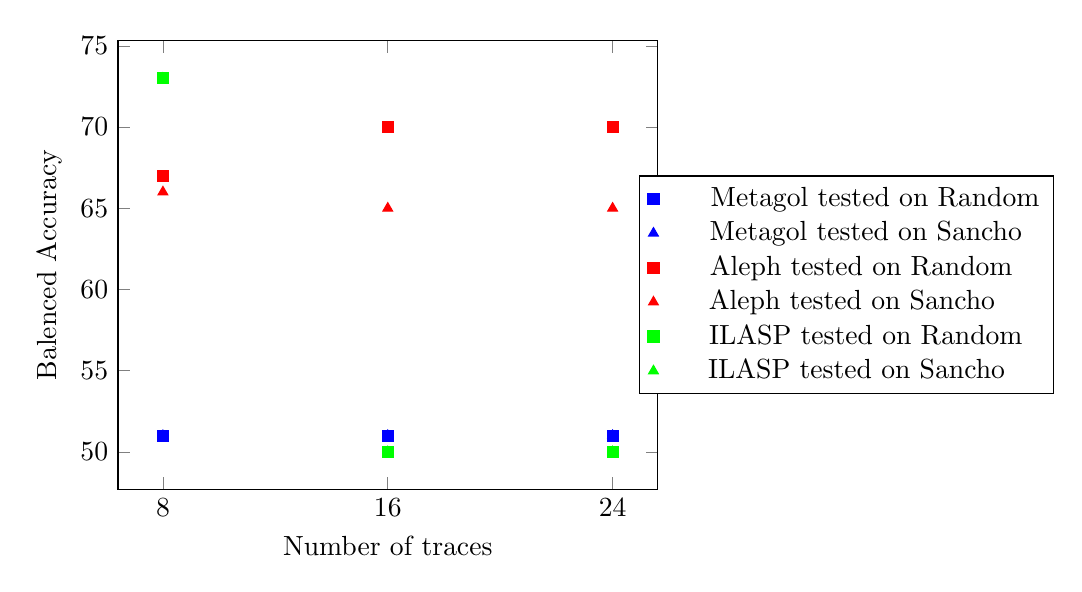
\begin{tikzpicture}
\begin{axis}[scatter/classes={
	a1={mark=square*,blue},%
	a2={mark=triangle*,blue},%
	b1={mark=square*,red},%
	b2={mark=triangle*,red},%
	c1={mark=square*,green},%
	c2={mark=triangle*,green}},
legend style={at={(1.35,0.7)},
	anchor=north},
xtick=data,
ylabel={Balenced Accuracy},
xlabel={Number of traces}]
\addplot[scatter,only marks,
scatter src=explicit symbolic] coordinates {
	(8,51)     	[a1]
	(8,51)     	[a2]
	(16,51)    	[a1]
	(16,51)    	[a2]
	(24,51)    	[a1]
	(24,51)		[a2]
	(8,67)		[b1]
	(8,66)		[b2]
	(16,70)		[b1]
	(16,65)		[b2]
	(24,70)		[b1]
	(24,65)		[b2]
	(8,73)		[c1]
	(8,73)		[c2]
	(16,50)		[c1]
	(16,50)		[c2]
	(24,50)		[c1]
	(24,50)		[c2]
};
\legend{\ \ \ \ \ Metagol tested on Random,\ \ \ Metagol tested on Sancho,\ \ Aleph tested on Random,Aleph tested on Sancho, \ \ \ ILASP tested on Random,\ ILASP tested on Sancho,d}
\end{axis}
\end{tikzpicture}
\\\\
When ILASP and Metagol have not had enough time to learn a predicate they output nothing. Both systems scale exponentially in time taken according to the size of the input. Whilst for Metagol it didn't have time even for the 8 traces ILASP ran out of time only on the 16 and 24 traces training sets. This had the effect for ILASP of a large drop in effectiveness. For 16 and 24 the default program consisting of just \textit{true} was used. This gave the balanced accuracy of 50 for each predicate. Metagol still managed to learn the simple predicates that it had managed on the 8 trace training set however did not increase at all in effectiveness over the rest of the experiment.

Unlike the other systems Aleph was consistently able to process the entire input since its method of learning is less computationally intense. When tested on the random traces Aleph did better with the increased number of traces. This was most likely due to the fact that more cases were encountered in the training data. Since Aleph usually ends up putting the cases it encounters straight into the program this simply meant there was a greater number of situations in the testing set that Aleph had seen before and was thus correctly able to classify. When tested on the optimal traces Aleph got worse. This is possibly due to the maximum size of Aleph programs taking effect. The clauses relevant to the optimal traces may be pushed out of the program by the vast number of clauses taken from the random gameplay examples.

If this experiment were to be conducted again much more enlightening results than these could be obtained by increasing the time given to each system to learn each predicate or even using a system with greater computational power to run the experiments. 


